% Graphical abstract: AI-rendered artwork (ga_background.png, no text) + TikZ text overlay.
% Labels sit only in empty zones of the artwork. Numbers: ledger A-006 (MAE), A-017 (median rho
% under source-paper holdout). The rho bars are redrawn to scale (0.34 : 0.17 = 2 : 1) because the
% artwork's bars are not proportional to the data.
% Working asset: author checks at 13 x 5 cm before submission.
\documentclass[tikz,border=0pt]{standalone}
\usepackage[T1]{fontenc}
\usepackage{lmodern}
\definecolor{ink}{HTML}{18344C}
\definecolor{teal}{HTML}{16677B}
\definecolor{slate}{HTML}{526676}
\definecolor{bargrey}{HTML}{7A8590}
\begin{document}
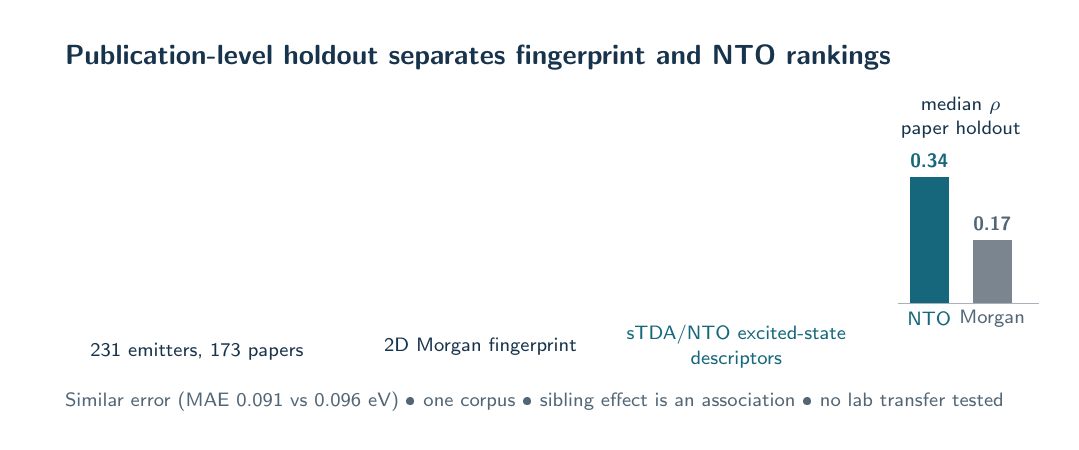
\begin{tikzpicture}[x=1cm,y=1cm]
  \useasboundingbox (0,0) rectangle (13,5);
  \fill[white] (0,0) rectangle (13,5);
  \IfFileExists{ga_background.png}{\node[anchor=south west,inner sep=0pt] at (0,0)
    {\includegraphics[width=13cm,height=5cm]{ga_background.png}};}{}

  % Title band (above the artwork's navy rule at y ~ 4.25)
  \node[anchor=west,font=\sffamily\bfseries\fontsize{10}{12}\selectfont,text=ink] at (0.35,4.62)
    {Publication-level holdout separates fingerprint and NTO rankings};

  % Labels under each artwork zone (free band y ~ 0.9--1.3)
  \node[align=center,text=ink,font=\sffamily\fontsize{7.5}{9}\selectfont] at (2.15,0.88)
    {231 emitters, 173 papers};
  \node[align=center,text=ink,font=\sffamily\fontsize{7.5}{9}\selectfont] at (5.75,0.95)
    {2D Morgan fingerprint};
  \node[align=center,text=teal,font=\sffamily\fontsize{7.5}{9}\selectfont] at (9.0,0.95)
    {sTDA/NTO excited-state\\descriptors};

  % Bars redrawn to scale over the artwork's bars
  \fill[white] (10.70,1.35) rectangle (12.98,3.75);
  \draw[slate!50,line width=.5pt] (11.05,1.5)--(12.85,1.5);
  \fill[teal]    (11.20,1.5) rectangle (11.70,3.10);   % NTO    rho 0.34 -> 1.60 cm
  \fill[bargrey] (12.00,1.5) rectangle (12.50,2.30);   % Morgan rho 0.17 -> 0.80 cm
  \node[text=teal,font=\sffamily\bfseries\fontsize{7.5}{9}\selectfont] at (11.45,3.31) {0.34};
  \node[text=slate,font=\sffamily\bfseries\fontsize{7.5}{9}\selectfont] at (12.25,2.51) {0.17};
  \node[text=teal,font=\sffamily\fontsize{7}{8}\selectfont] at (11.45,1.30) {NTO};
  \node[text=slate,font=\sffamily\fontsize{7}{8}\selectfont] at (12.25,1.30) {Morgan};
  \node[align=center,text=ink,font=\sffamily\fontsize{7}{8.5}\selectfont] at (11.85,3.86)
    {median $\rho$\\paper holdout};

  % Footer (free band y < 0.6)
  \node[anchor=west,text=slate,font=\sffamily\fontsize{6.8}{8.5}\selectfont] at (0.35,0.25)
    {Similar error (MAE 0.091 vs 0.096 eV) \textbullet{} one corpus \textbullet{} sibling effect is an association \textbullet{} no lab transfer tested};
\end{tikzpicture}
\end{document}
